
\chapter{محرمانگی تفاضلی موضعی}
\label{sec:ldp}

\section{مقدمه}
در فصل پیشین (\ref{ch:preliminaries})، مفاهیم بنیادی نظریه اندازه و مدل محرمانگی تفاضلی متمرکز (\lr{CDP}) را بررسی کردیم. 
همان‌طور که در بخش \ref{sec:bg:cdp} مشاهده شد، مدل متمرکز (\lr{CDP}) بر فرض وجود یک متصدی مورد اعتماد استوار است که به داده‌های خام تمامی کاربران دسترسی دارد ($M: \Xset^n \to \Rset$).
اگرچه این مدل دقت آماری بالایی را فراهم می‌کند، اما ذخیره‌سازی متمرکز داده‌ها یک «نقطه شکست مرکزی» ایجاد می‌کند؛ به این معنا که نفوذ به سرور یا خیانت متصدی، حریم خصوصی تمامی کاربران را به خطر می‌اندازد.
برای مثال در بسیاری از کاربردهای مدرن، مانند جمع‌آوری داده‌های تله‌متری مرورگرها یا اپلیکیشن‌های موبایل، اعتماد به سرور مرکزی خطرات امنیتی و چالش‌های حقوقی را به همراه دارد.

در پاسخ به این چالش، مدل «محرمانگی تفاضلی موضعی»\LTRfootnote{Local Differential Privacy} یا به اختصار \lr{LDP} پارادایم اعتماد را تغییر می‌دهد. 
در این مدل، هیچ موجودیتی (حتی سرور) به داده‌ی خام $X_i$ دسترسی ندارد؛ بلکه هر کاربر به صورت مستقل مکانیزم تصادفی $\mech_i$ را روی داده‌ی خود اجرا کرده و تنها خروجی نویزدار $Z_i$ را منتشر می‌کند (شکل \ref{fig:ldp-model}).

% \begin{figure}[ht]
% 	\centering
% 	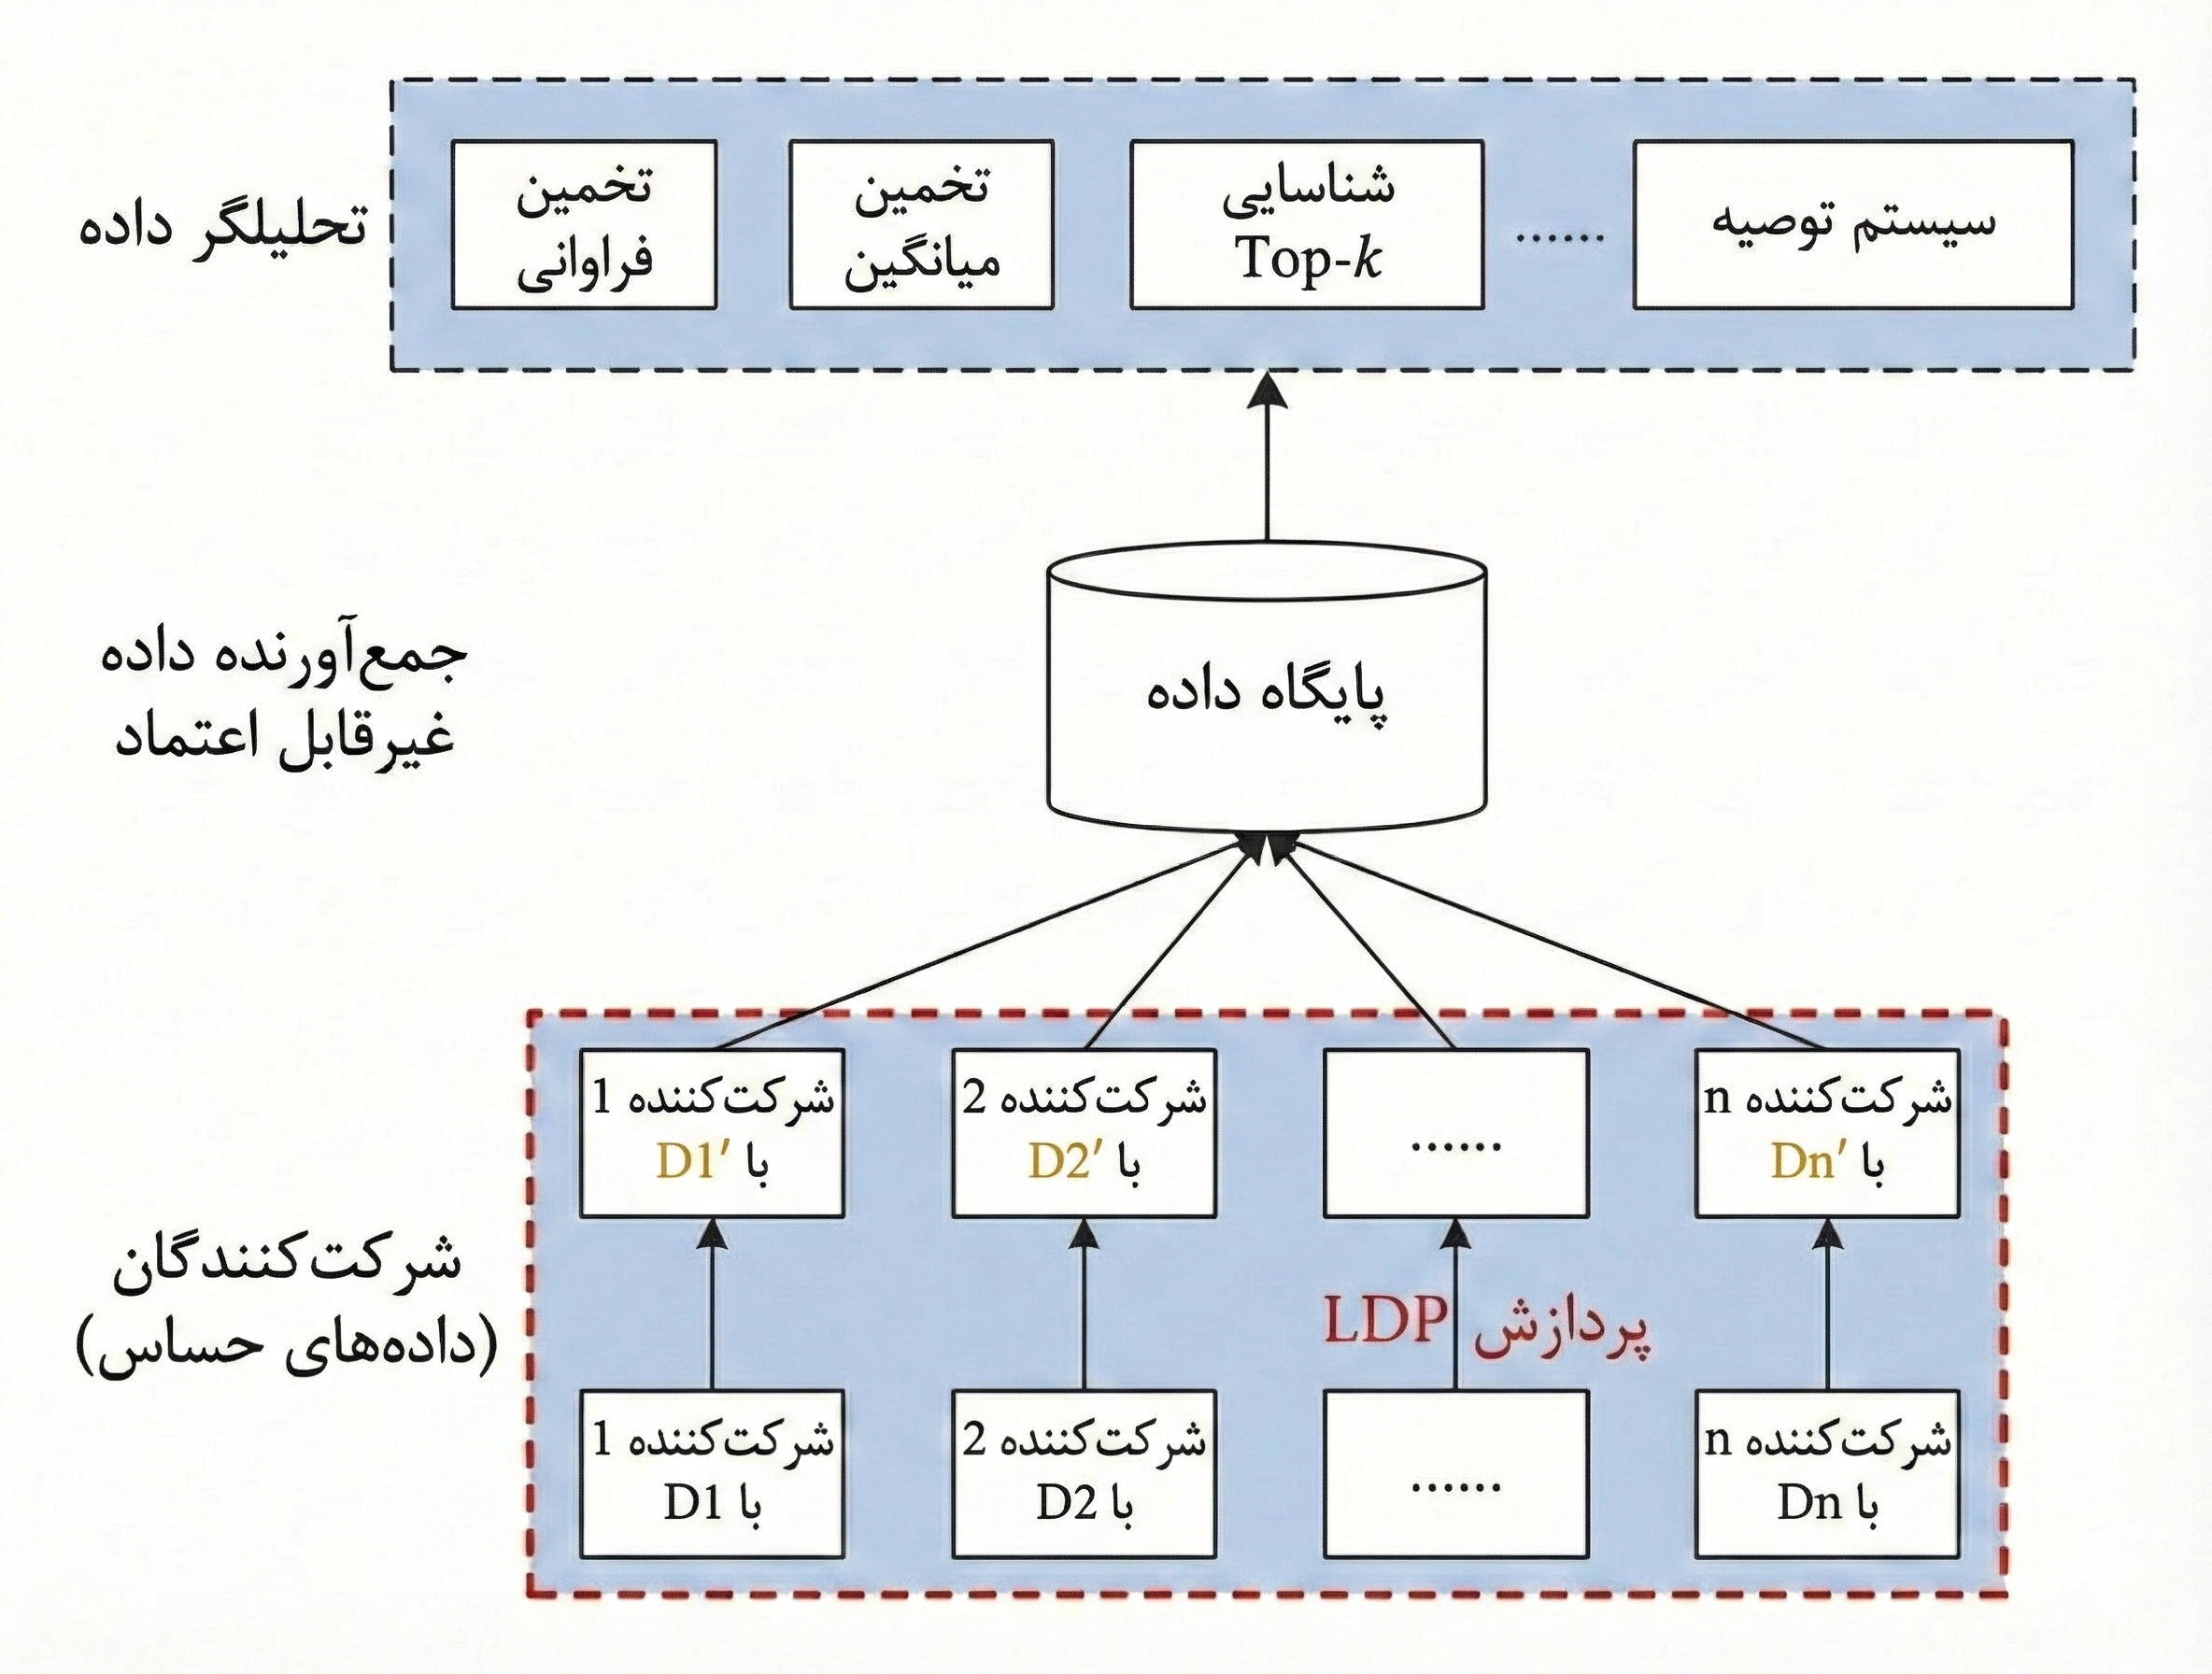
\includegraphics[width=0.7\textwidth]{figs/LDP.png}
% 	\caption{گذار از مدل متمرکز به موضعی؛ نویز به صورت محلی (\lr{Local}) روی دستگاه کاربر اضافه می‌شود.}
% 	\label{fig:ldp-model}
% \end{figure}
\begin{figure}[ht]
	
    \centering
    \begin{tikzpicture}[
        node distance=2.5cm,
        box/.style={rectangle, draw, minimum width=2.2cm, minimum height=1.5cm, align=center, thick},
        smallbox/.style={rectangle, draw, minimum width=1.5cm, minimum height=1cm, align=center, thick},
        arrow/.style={-stealth, thick},
        user/.style={inner sep=0pt, minimum size=1.5cm}
    ]

    % --- Level 1: Individuals (افراد) ---
    \node[above=0.5cm of u1] {\rl{افراد (داده‌ها)}};

    \node[user] (u1) at (0, 2.5) {\scalebox{3}{\smiley}};
    \node[user] (u2) at (0, 0.5) {\scalebox{3}{\smiley}};
    \node at (0, -0.7) {\Huge $\vdots$};
    \node[user] (un) at (0, -2) {\scalebox{3}{\smiley}};

    % --- Level 2: Local DP Mechanisms (مکانیزم‌های موضعی) ---
    \node (m1) [smallbox, right of=u1, xshift=1cm] {\rl{مکانیزم} \\ \lr{DP}};
    \node (m2) [smallbox, right of=u2, xshift=1cm] {\rl{مکانیزم} \\ \lr{DP}};
    \node (mn) [smallbox, right of=un, xshift=1cm] {\rl{مکانیزم} \\ \lr{DP}};

    % --- Level 3: Trusted Curator / Aggregator (تجمیع‌کننده) ---
    \node (curator) [box, right of=m2, xshift=3cm, yshift=0.2cm] {\rl{متصدی مورد اعتماد} \\ \rl{کارشناس محرمانگی}};
    \node[above=0.1cm of curator, font=\small] {\rl{نتایج خصوصی‌شده}};

    % --- Level 4: Public (انتشار عمومی) ---
    \node (public) [smallbox, right of=curator, xshift=2.5cm] {\rl{عمومی}};

    % --- Arrows and Labels ---
    \draw [arrow] (u1.east) -- node[above, font=\footnotesize] {$X_1$} (m1);
    \draw [arrow] (u2.east) -- node[above, font=\footnotesize] {$X_2$} (m2);
    \draw [arrow] (un.east) -- node[above, font=\footnotesize] {$X_n$} (mn);
    
    \draw [arrow] (m1.east) -- node[above, pos=0.4, font=\footnotesize] {$Z_1$} (curator.145);
    \draw [arrow] (m2.east) -- node[above, pos=0.4, font=\footnotesize] {$Z_2$} (curator.180);
    \draw [arrow] (mn.east) -- node[above, pos=0.4, font=\footnotesize] {$Z_n$} (curator.215);

    \draw [arrow] (curator) -- node[above, align=center, font=\footnotesize] {\rl{پس‌پردازش} \\ \rl{و انتشار}} (public);

    \end{tikzpicture}
	\caption{\rl{گذار از مدل متمرکز به موضعی؛ نویز به صورت محلی (\lr{Local}) روی دستگاه کاربر اضافه می‌شود.}}
\label{fig:ldp-model}
\end{figure}

\section{تعاریف رسمی و مدل‌های محاسباتی}
\label{sec:ldp:definitions}

در مدل موضعی، مجموعه‌ای از $n$ کاربر وجود دارند که هر کدام داده‌ای خصوصی $X_i \in \Xset$ در اختیار دارند. برخلاف مدل متمرکز که شرط محرمانگی روی «پایگاه‌داده‌های همسایه» تعریف می‌شد، در این‌جا شرط محرمانگی باید برای «هر جفت ورودی ممکن» در دامنه برقرار باشد تا تمایز قائل شدن بین مقادیر مختلف ورودی برای مهاجم دشوار گردد.

\begin{تعریف}[تصادفی‌ساز موضعی\LTRfootnote{Local Randomizer}]
\label{def:local-randomizer}
یک مکانیزم تصادفی $\mech: \Xset \to \Zset$ را یک تصادفی‌ساز موضعی می‌نامیم که ورودی $x \in \Xset$ را دریافت کرده و خروجی $z \in \Zset$ را بر اساس توزیع احتمال شرطی $Q(z|x)$ تولید می‌کند.
\end{تعریف}

\subsection{تعریف ریاضی \lr{LDP}}

هسته‌ی اصلی این مدل، تضمین این نکته است که توزیع‌های خروجی برای هر دو ورودی متمایز، از نظر آماری بسیار به هم نزدیک باشند.

\begin{تعریف}[\LDP]
\label{def:alpha-ldp}
یک مکانیزم تصادفی \mech، \LDP \ است، اگر برای تمام جفت ورودی‌های $x, x' \in \Xset$ و برای هر رویداد خروجی $\Sset \subseteq \Zset$ (در $\sigma$-جبرِ برد) داشته باشیم:
\begin{equation}
\label{eq:ldp-def-sup}
\sup_{x, x' \in \Xset} \sup_{\Sset \subseteq \Zset} \frac{\Pr[\mech(x) \in \Sset]}{\Pr[\mech(x') \in \Sset]} \le e^{\al}
\end{equation}
\end{تعریف}

\textbf{نکته:} در متون آماری این حوزه (مانند \cite{Duchi2013})، معمولاً از پارامتر \al \ برای بودجه‌ی محرمانگی موضعی استفاده می‌شود تا تمایز آن با پارامتر \eps \ در مدل متمرکز مشخص گردد. ما نیز در این فصل و فصول بعدی از این نمادگذاری پیروی می‌کنیم.

این تعریف را می‌توان با استفاده از مفهوم «واگرایی ماکزیمم» ($D_\infty$) که پیش‌تر معرفی شد، به صورت فشرده‌تری بیان کرد. شرط \eqref{eq:ldp-def-sup} دقیقاً معادل است با:
\begin{equation}
\label{eq:ldp-dinf}
\sup_{x, x' \in \Xset} D_\infty(Q(\cdot|x) \parallel Q(\cdot|x')) \le \al
\end{equation}
این رابطه نشان می‌دهد که \LDP \ محدودیتی سخت‌گیرانه بر روی «نسبت درست‌نمایی»\LTRfootnote{Likelihood Ratio} توزیع‌های خروجی اعمال می‌کند و تضمین می‌دهد که مشاهده‌ی خروجی $z$، اطلاعات اندکی درباره‌ی ورودی $x$ افشا می‌کند.

\subsection{محرمانگی تقریبی}

مشابه مدل متمرکز، در برخی کاربردها نیاز است که تعریف \LDP \ را تضعیف کنیم تا اجازه‌ی یک احتمال شکست ناچیز $\delta$ داده شود. این حالت معمولاً زمانی رخ می‌دهد که دامنه یا برد مکانیزم نامتناهی باشد (مانند مکانیزم گوسی).

\begin{تعریف}[\lr{$(\al, \del)$-LDP}]
\label{def:approx-ldp}
یک مکانیزم \mech دارای محرمانگی تفاضلی موضعی تقریبی است اگر برای تمام ورودی‌های $x, x' \in \Xset$ و تمام زیرمجموعه‌های خروجی $\Sset \subseteq \Zset$ داشته باشیم:
\begin{equation}
\Pr[\mech(x) \in \Sset] \le e^{\al} \cdot \Pr[\mech(x') \in \Sset] + \delta
\end{equation}
بدیهی است که اگر $\delta=0$ باشد، این تعریف به حالت \LDP \ خالص باز می‌گردد \cite{Wang2020}.
\end{تعریف}


\section{پروتکل‌های تعاملی و خواص ترکیب}
\label{sec:ldp:interaction}

برای تحلیل دقیق حدود مینیماکس و درک محدودیت‌های بنیادین \lr{LDP}، نیازمند مدل‌سازی دقیق نحوه‌ی تعامل کاربران با سرور (یا جمع‌آورنده داده) هستیم. دوچی و همکاران \cite{Duchi2013} پروتکل‌های موضعی را بر اساس ساختار وابستگی آماری خروجی‌ها به دو دسته‌ی کلی تقسیم می‌کنند: غیرتعاملی و تعاملی.

\subsection{پروتکل‌های غیرتعاملی}
در پروتکل‌های غیرتعاملی\LTRfootnote{Non-interactive}، تمام کاربران $i=1, \dots, n$ مکانیزم‌های خود را به صورت هم‌زمان و مستقل از یک‌دیگر اجرا می‌کنند. اگر $Z_i$ خروجی کاربر $i$-ام باشد، توزیع آن تنها به داده‌ی خصوصی $X_i$ وابسته است و هیچ وابستگی‌ای به خروجی سایر کاربران ندارد.
به بیان ریاضی، توزیع مشترک خروجی‌ها به صورت حاصل‌ضرب توزیع‌های حاشیه‌ای فاکتور می‌شود:
\begin{equation}
\Pr(Z_1, \dots, Z_n | X_1, \dots, X_n) = \prod_{i=1}^n Q_i(Z_i | X_i)
\end{equation}
بسیاری از پیاده‌سازی‌های صنعتی فعلی، از جمله \lr{RAPPOR} گوگل \cite{Erlingsson2014}، در این دسته قرار می‌گیرند.

\subsection{پروتکل‌های تعاملی (ترتیبی)}
در پروتکل‌های تعاملی\LTRfootnote{Interactive / Sequential}، کاربران به نوبت داده‌های خود را ارسال می‌کنند و مکانیزم کاربر $i$-ام می‌تواند به خروجی‌های مشاهده‌شده از کاربران پیشین ($Z_1, \dots, Z_{i-1}$) وابسته باشد. این مدل، آزادی عمل بیشتری را برای طراحی الگوریتم‌های تطبیقی فراهم می‌کند.

از دیدگاه آنالیز ریاضی، این فرآیند با استفاده از «کرنل‌های احتمالاتی»\LTRfootnote{Probability Kernels} مدل‌سازی می‌شود. فرض کنید $Z_{1:i-1} = (Z_1, \dots, Z_{i-1})$ بردار خروجی‌های پیشین باشد که $\sigma$-فیلد $\mathcal{F}_{i-1}$ را تولید می‌کند. مکانیزم کاربر $i$-ام، یک کرنل احتمالاتی $Q_i$ است که خروجی $Z_i \in \Zset$ را مشروط بر داده‌ی خصوصی $X_i$ و تاریخچه‌ی عمومی $Z_{1:i-1}$ تولید می‌کند:
\begin{equation}
Z_i \sim Q_i(dz_i | x_i, z_{1:i-1})
\end{equation}
شرط اساسی محرمانگی در اینجا این است که با شرطی‌سازی روی $X_i$ و $Z_{1:i-1}$، متغیر $Z_i$ باید از سایر داده‌های خصوصی $X_{j \neq i}$ مستقل باشد (شرط مارکوفی). این ساختار به پروتکل اجازه می‌دهد تا پارامترهای پرس‌وجو را به صورت پویا بر اساس اطلاعات کسب‌شده از کاربران قبلی تنظیم کند.

\subsection{قضیه ترکیب ترتیبی}
یکی از ویژگی‌های بنیادین \lr{LDP}، پایداری آن در برابر ترکیب است. اگر یک پروتکل شامل چندین مرحله‌ی تعاملی باشد، بودجه‌های محرمانگی با یک‌دیگر جمع می‌شوند. قضیه‌ی زیر، کران بالای محرمانگی را برای یک پروتکل ترتیبی بیان می‌کند \cite{Duchi2013}.

\begin{قضیه}[ترکیب ترتیبی\LTRfootnote{Sequential Composition}]
\label{thm:ldp-composition}
فرض کنید در یک پروتکل تعاملی، برای هر کاربر $i \in \{1, \dots, n\}$ و به ازای هر تاریخچه‌ی ممکن $z_{1:i-1} \in \Zset^{i-1}$، مکانیزم $Q_i(\cdot | \cdot, z_{1:i-1})$ دارای خاصیت \LDP[\al_i] نسبت به ورودی $x_i$ باشد. آنگاه توزیع مشترک کل خروجی‌ها ($Z_1, \dots, Z_n$)، دارای محرمانگی تفاضلی موضعی با بودجه‌ی مجموع است:
\begin{equation}
\al_{total} = \sum_{i=1}^n \al_i
\end{equation}
\end{قضیه}

\begin{اثبات}
اثبات بر پایه خاصیت زنجیره‌ای واگرایی ماکزیمم ($D_\infty$) یا تجزیه‌ی نسبت‌های درست‌نمایی استوار است. اگر $P$ و $P'$ دو توزیع احتمال روی دنباله‌ی خروجی‌ها $Z^n$ باشند که ناشی از دو دنباله ورودی $x^n$ و ${x'}^n$ هستند، نسبت احتمال توأم به حاصل‌ضرب نسبت‌های شرطی تجزیه می‌شود:
\[
\frac{P(z^n)}{P'(z^n)} = \prod_{i=1}^n \frac{Q_i(z_i | x_i, z_{1:i-1})}{Q_i(z_i | x'_i, z_{1:i-1})}
\]
از آن‌جا که هر گام طبق فرض با $e^{\al_i}$ کران‌دار است، کل حاصل‌ضرب با $e^{\sum \al_i}$ کران‌دار خواهد بود.
\end{اثبات}


\section{مکانیزم‌های پایه در \lr{LDP}}
\label{sec:ldp:mechanisms}

در این بخش، مکانیزم‌های بنیادین \lr{LDP} \ را با رویکردی آماری تحلیل می‌کنیم. هدف اصلی در طراحی این مکانیزم‌ها، یافتن نگاشتی تصادفی است که علاوه بر ارضای شرط محرمانگی، «خطای تخمین» (که معمولاً با واریانس سنجیده می‌شود) را کمینه کند. فرض بنیادی در تمام این مکانیزم‌ها این است که برای بازیابی اطلاعات آماری (مانند هیستوگرام)، از یک «تخمین‌گر نااریب»\LTRfootnote{Unbiased Estimator} معکوس استفاده می‌شود.


\subsection{پاسخ تصادفی دودویی \lr{(RR)}}
\label{sec:ldp:rr}

پایه‌ای‌ترین مکانیزم \LDP، پاسخ تصادفی\LTRfootnote{Randomized Response} (\lr{RR}) برای دامنه‌ی دودویی $\Xset = \{0, 1\}$ است. این مکانیزم را می‌توان به صورت یک کانال متقارن دودویی مدل‌سازی کرد که ورودی $x$ را با احتمال $p$ حفظ کرده و با احتمال $1-p$ قرینه می‌کند:
\begin{equation}
\Pr[y=z | x] = 
\begin{cases}
p & \text{if } \ \ z = x \\
1-p & \text{if } \ \ z \neq x
\end{cases}
\end{equation}

\textbf{اثبات \LDP:}
برای اینکه این مکانیزم شرط \LDP[\al] را برآورده کند، طبق تعریف \ref{def:alpha-ldp} باید نسبت درست‌نمایی برای هر دو ورودی متمایز $x, x'$ و هر خروجی ممکن $y$، با $e^\al$ کران‌دار شود. بدترین حالت زمانی رخ می‌دهد که صورت کسر بیشترین احتمال ($p$) و مخرج کسر کمترین احتمال ($1-p$) باشد:
\begin{equation}
\sup_{y \in \{0,1\}} \frac{\Pr[y|x]}{\Pr[y|x']} = \frac{p}{1-p} \le e^\al
\end{equation}
با حل این نامساوی برای $p$ (و با فرض $p > 1/2$ برای بی‌معنی نشدن نتیجه)، مقدار بهینه احتمال حفظ پاسخ برای بودجه‌ی \al \ به دست می‌آید:
\begin{equation}
p = \frac{e^\al}{e^\al + 1}
\end{equation}

\textbf{تحلیل واریانس:}
برای تحلیل دقیق خطا، ابتدا تخمین‌گر نااریب را استخراج می‌کنیم. اگر $y \in \{0, 1\}$ خروجی مکانیزم باشد، هدف یافتن تابعی $\hat{f}(y)$ است که $\Eset[\hat{f}(y)] = x$ باشد.

\begin{لم}[واریانس پاسخ تصادفی]
\label{lem:rr-variance}
برای مکانیزم \lr{RR} با پارامتر $p$، تخمین‌گر نااریب ورودی $x$ به صورت زیر است:
\begin{equation}
\hat{x} = \frac{y - (1-p)}{2p - 1}
\end{equation}
و واریانس این تخمین‌گر بر حسب بودجه محرمانگی \al \ برابر است با:
\begin{equation}
\mathrm{Var}[\hat{x}] = \frac{e^\al}{(e^\al - 1)^2}
\end{equation}
\end{لم}

\begin{اثبات}
ابتدا نااریبی را بررسی می‌کنیم. امید ریاضی $y$ برابر است با:
\[\Eset[y] = p \cdot x + (1-p)(1-x) = (2p-1)x + (1-p)\]
با جایگذاری در معادله تخمین‌گر:
\[
\Eset[\hat{x}] = \frac{\Eset[y] - (1-p)}{2p - 1} = \frac{(2p-1)x}{2p-1} = x
\]
برای محاسبه واریانس، چون $y$ یک متغیر برنولی است، واریانس آن $p(1-p)$ می‌شود. با اعمال خواص واریانس ($\mathrm{Var}[aY+b] = a^2\mathrm{Var}[Y]$) داریم:
\[
\mathrm{Var}[\hat{x}] = \frac{\mathrm{Var}[y]}{(2p-1)^2} = \frac{p(1-p)}{(2p-1)^2}
\]
حال با جایگذاری $p = \frac{e^\al}{e^\al+1}$ در رابطه بالا:
\[
\mathrm{Var}[\hat{x}] = \frac{\frac{e^\al}{(e^\al+1)^2}}{(\frac{2e^\al}{e^\al+1} - 1)^2} = \frac{\frac{e^\al}{(e^\al+1)^2}}{(\frac{e^\al-1}{e^\al+1})^2} = \frac{e^\al}{(e^\al-1)^2}
\]
\end{اثبات}

\subsection{پاسخ تصادفی تعمیم‌یافته \lr{(GRR)}}
\label{sec:ldp:grr}
پاسخ تصادفی تعمیم‌یافته\LTRfootnote{Generalized Randomized Response}،
برای دامنه‌های گسسته با $k > 2$ عنصر ($\Xset = \{1, \dots, k\}$)، به عنوان تعمیم مستقیم \lr{RR} معرفی می‌شود. این مکانیزم را می‌توان با یک «ماتریس گذار»\LTRfootnote{Transition Matrix} تصادفی $\mathbf{Q} \in [0,1]^{k \times k}$ توصیف کرد.

\begin{تعریف}[ماتریس احتمال \lr{GRR}]
در مکانیزم \lr{GRR}، ماتریس احتمال شرطی $\mathbf{Q}$ که درایه $(i,j)$ آن برابر با $\Pr[z=j | x=i]$ است، به صورت زیر تعریف می‌شود:
\begin{equation}
\mathbf{Q} = 
\begin{pmatrix}
p & q & \dots & q \\
q & p & \dots & q \\
\vdots & \vdots & \ddots & \vdots \\
q & q & \dots & p
\end{pmatrix}_{k \times k}
\end{equation}
که در آن $p$ احتمال گزارش صادقانه و $q$ احتمال گزارش هر یک از $k-1$ گزینه‌ی دیگر است.
\end{تعریف}

به صورت مشابه \lr{RR} می‌توان نشان داد که
مقادیر بهینه برای ارضای شرط \LDP[\al] عبارتند از:
\begin{equation}
p = \frac{e^\al}{e^\al + k - 1}, \quad q = \frac{1}{e^\al + k - 1}
\end{equation}

برای تخمین فراوانی یک آیتم خاص $v \in \Xset$، از تخمین‌گر نااریب $\hat{c}_v = \frac{\mathbb{I}(z=v) - q}{p-q}$ استفاده می‌شود. با تحلیلی مشابه لم \ref{lem:rr-variance}، واریانس این تخمین‌گر برابر خواهد بود با:
\begin{equation}
\label{eq:grr-var-derivation}
\mathrm{Var}_{GRR} = \frac{p(1-p)}{(p-q)^2} = \frac{(e^\al)(k-1) + (k-1)^2}{(e^\al - 1)^2} \approx \mathcal{O}(k)
\end{equation}
این رابطه نشان می‌دهد که واریانس \lr{GRR} وابستگی خطی به اندازه دامنه $k$ دارد که نقطه ضعف این روش در ابعاد بالاست.


\subsection{مکانیزم‌های مبتنی بر کدگذاری یگانی (\lr{UE})}
\label{sec:ldp:ue}

برای غلبه بر مشکل کاهش دقت \lr{GRR} در دامنه‌های بزرگ، خانواده‌ای از مکانیزم‌ها تحت عنوان «کدگذاری یگانی»\LTRfootnote{Unary Encoding (UE)} توسعه یافته‌اند. این رویکرد اساس پروتکل مشهور \lr{RAPPOR} گوگل را تشکیل می‌دهد \cite{Erlingsson2014, Wang2020}.


\begin{تعریف}[کدگذاری یگانی]
در این روش، فرآیند خصوصی‌سازی طی دو مرحله انجام می‌شود:
\begin{enumerate}
    \item \textbf{کدگذاری قطعی:} ورودی $x \in \{1, \dots, k\}$ به یک بردار بیتی $v \in \{0, 1\}^k$ تبدیل می‌شود که تنها در موقعیت $x$ برابر با ۱ و در سایر جاها ۰ است (\lr{One-hot encoding}).
    \item \textbf{اختلال\LTRfootnote{Perturbation} مستقل:} هر بیت این بردار به صورت مستقل با استفاده از یک مکانیزم باینری معکوس می‌شود. اگر $v_i$ بیت $i$-ام بردار کدگذاری شده باشد، خروجی \ $z_i$ به صورت زیر تولید می‌شود:
    \begin{equation}
    \Pr[z_i = 1] = 
    \begin{cases} 
    p & \text{if } \ \ v_i = 1 \\
    q & \text{if } \ \ v_i = 0
    \end{cases}
    \end{equation}
\end{enumerate}
\end{تعریف}

\begin{مثال}
فرض کنید دامنه شامل ۴ آیتم باشد ($\Xset = \{1, 2, 3, 4\}$) و ورودی کاربر $x=2$ باشد.
\begin{enumerate}
    \item بردار کدگذاری شده: $v = [0, 1, 0, 0]$
    \item اعمال نویز: هر بیت مستقل پرتاب می‌شود. ممکن است خروجی نهایی $z = [0, 1, 1, 0]$ شود (بیت سوم از ۰ به ۱ تغییر کرده است).
\end{enumerate}
\end{مثال}

\textbf{اثبات \LDP:}
برای بررسی شرط \LDP[\al]، نسبت احتمال خروجی برداری $z = (z_1, \dots, z_k)$ را برای دو ورودی متمایز $x$ و $x'$ محاسبه می‌کنیم. بردارهای متناظر $v$ و $v'$ تنها در دو موقعیت تفاوت دارند: موقعیت $x$ (که $v_x=1, v'_x=0$) و موقعیت $x'$ (که $v_{x'}=0, v'_{x'}=1$). در سایر موقعیت‌ها ($j \neq x, x'$) بیت‌ها یکسان و برابر صفر هستند و در نسبت احتمالات ساده می‌شوند.
از آنجا که بیت‌ها مستقل هستند:
\begin{equation}
\frac{\Pr[z|x]}{\Pr[z|x']} = \frac{\Pr[z_x|v_x=1]}{\Pr[z_x|v'_x=0]} \cdot \frac{\Pr[z_{x'}|v_{x'}=0]}{\Pr[z_{x'}|v'_{x'}=1]}
\end{equation}
بیشینه‌ی این کسر زمانی رخ می‌دهد که صورت کسر ماکزیمم و مخرج مینیمم شود؛ یعنی زمانی که $z_x=1$ (حفظ بیت ۱) و $z_{x'}=0$ (حفظ بیت ۰) باشد. در این حالت:
\begin{equation}
\frac{\Pr[z|x]}{\Pr[z|x']} \le \frac{p}{q} \cdot \frac{1-q}{1-p} = \frac{p(1-q)}{q(1-p)}
\end{equation}
بنابراین شرط \LDP[\al] معادل است با:
\begin{equation}
\label{eq:ue-ldp-condition}
\al = \ln \left( \frac{p(1-q)}{q(1-p)} \right)
\end{equation}

\begin{لم}[تحلیل واریانس \lr{UE}]
در پروتکل‌های \lr{UE}، واریانس تخمین فراوانی برای هر آیتم، تنها به پارامترهای $p$ و $q$ وابسته است و از رابطه زیر پیروی می‌کند:
\begin{equation}
\mathrm{Var}_{UE} = \frac{q(1-q)}{(p-q)^2}
\end{equation}
(نکته: این واریانس برای حالتی است که ورودی واقعی کاربر آن آیتم نباشد، که در دامنه‌های بزرگ حالت غالب است).
\end{لم}

دو استراتژی اصلی برای تنظیم $p$ و $q$ بر اساس رابطه \eqref{eq:ue-ldp-condition} وجود دارد:

\textbf{۱. کدگذاری یگانی متقارن (\lr{SUE}):}
در این روش $p+q=1$ در نظر گرفته می‌شود. با جایگذاری در شرط \LDP، مقادیر بهینه عبارتند از $p = \frac{e^{\al/2}}{e^{\al/2}+1}$ و $q = \frac{1}{e^{\al/2}+1}$. واریانس در این حالت برابر است با:
\begin{equation}
\mathrm{Var}_{SUE} = \frac{e^{\al/2}}{(e^{\al/2}-1)^2}
\end{equation}

\textbf{۲. کدگذاری یگانی بهینه (\lr{OUE}):}
وانگ و همکاران \cite{Wang2020} نشان دادند که برای کمینه‌سازی واریانس در دامنه‌های بزرگ، باید اطلاعات بیت‌های ۱ (سیگنال) حفظ شود ($p=1/2$) و نویز روی بیت‌های ۰ (که اکثر بردار را تشکیل می‌دهند) کنترل شود ($q = \frac{1}{e^\al+1}$).
واریانس حاصل برابر است با:
\begin{equation}
\mathrm{Var}_{OUE} = \frac{4e^\al}{(e^\al-1)^2}
\end{equation}
\subsection{تحلیل مقایسه‌ای: چرا \lr{GRR} در ابعاد بالا شکست می‌خورد؟}
\label{sec:comparison-grr-oue}

یکی از مهم‌ترین نتایج نظری در ادبیات \lr{LDP}، مقایسه رفتار مجانبی \lr{GRR} و \lr{OUE} نسبت به اندازه دامنه $k$ است.

\begin{مثال}[ناکارآمدی \lr{GRR} در دامنه‌های بزرگ]
فرض کنید می‌خواهیم کلمات پرکاربرد را از یک لغت‌نامه با $k=100,000$ کلمه استخراج کنیم.
\begin{itemize}
    \item در مکانیزم \lr{GRR}، طبق رابطه \eqref{eq:grr-var-derivation}، واریانس تقریباً با $k$ رشد می‌کند:
    \[ \mathrm{Var}_{GRR} \approx \frac{k}{(e^\al-1)^2} \]
    به عبارتی، نویز اضافه شده متناسب با کل اندازه دیکشنری است که سیگنال کلمات نادر را کاملاً محو می‌کند.
    
    \item در مکانیزم \lr{OUE}، واریانس مستقل از $k$ است:
    \[ \mathrm{Var}_{OUE} = \frac{4e^\al}{(e^\al-1)^2} \]
\end{itemize}
این استقلال از $k$ باعث می‌شود که خانواده \lr{UE} گزینه‌ی برتر برای دامنه‌های بزرگ باشند. با این حال، \lr{OUE} هزینه مخابراتی بالایی دارد (ارسال بردار با طول $k$). برای رفع این مشکل، نسخه بهبودیافته‌ای به نام «درهم‌سازی موضعی بهینه\LTRfootnote{Optimized Local Hashing (OLH)}»  توسط وانگ و همکاران \cite{Wang2017} معرفی شده است. این روش با استفاده از توابع درهم‌ساز، ورودی را فشرده کرده و بدون افزایش واریانس، هزینه مخابراتی را کاهش می‌دهد.
\end{مثال}


\subsection{مکانیزم لاپلاس موضعی}
\label{sec:ldp:laplace}


برای داده‌های عددی پیوسته، رویکرد استاندارد تعمیم مکانیزم لاپلاس از مدل متمرکز به مدل موضعی است. فرض کنید دامنه ورودی یک بازه‌ی کران‌دار $\Xset \subset \mathbb{R}$ باشد.
بدون کاستن از کلیت\LTRfootnote{Without Loss of Generality}، فرض می‌کنیم داده‌ها با یک تبدیل خطی به بازه‌ی $[-1, 1]$ نگاشت شده‌اند.
در مدل موضعی، شرط محرمانگی باید برای هر جفت ورودی $x, x' \in \Xset$ برقرار باشد. بنابراین «حساسیت سراسری» ($\Delta$) برابر با قطر دامنه است. در این صورت \Del، بیشترین مقدار ممکن را خواهد داشت:
\begin{equation}
\Delta = \sup_{x, x' \in [-1, 1]} |x - x'| = |1 - (-1)| = 2
\end{equation}

\begin{تعریف}[مکانیزم لاپلاس موضعی]
مکانیزم $\mech_{Lap}$ ورودی نرمالایز شده $x \in [-1, 1]$ را دریافت کرده و خروجی $z$ را طبق رابطه زیر تولید می‌کند:
\begin{equation}
z = x + \eta, \quad \eta \sim \mathrm{Lap}\left( \frac{\Delta}{\al} \right) = \mathrm{Lap}\left( \frac{2}{\al} \right)
\end{equation}
تابع چگالی احتمال \lr{(PDF)} خروجی برای ورودی $x$ به صورت زیر است:
\begin{equation}
f(z|x) = \frac{\al}{4} \exp\left( -\frac{\al |z-x|}{2} \right)
\end{equation}
\end{تعریف}

\textbf{اثبات \LDP:}
برای هر دو ورودی $x, x'$ و هر خروجی $z$، نسبت چگالی‌ها عبارت است از:
\begin{align}
\frac{f(z|x)}{f(z|x')} &= \frac{\exp(-\frac{\al}{2}|z-x|)}{\exp(-\frac{\al}{2}|z-x'|)} \\
&= \exp\left( \frac{\al}{2} (|z-x'| - |z-x|) \right)
\end{align}
طبق نامساوی مثلثی معکوس ($|a| - |b| \le |a-b|$):
\[
|z-x'| - |z-x| \le |(z-x') - (z-x)| = |x-x'| \le 2
\]
بنابراین نسبت احتمال با $\exp(\frac{\al}{2} \cdot 2) = e^\al$ کران‌دار می‌شود.

\begin{مثال}
فرض کنید می‌خواهیم دمای بدن یک بیمار را گزارش کنیم. اگر دامنه تغییرات دما $[35, 42]$ درجه باشد، طول بازه $42-35=7$ است.
اگر بدون نرمال‌سازی از لاپلاس استفاده کنیم، باید نویزی متناسب با $\frac{7}{\al}$ اضافه کنیم.
اما در روش استاندارد، ابتدا دما را به $[-1, 1]$ نگاشت می‌کنیم (که حساسیت ۲ شود)، نویز با مقیاس $\frac{2}{\al}$ اضافه می‌کنیم و در سمت سرور مجدداً نتیجه را به مقیاس اصلی برمی‌گردانیم.
حال اگر بخواهیم دمای بدن یک بیمار را که به بازه $[-1, 1]$ نرمالایز شده است، با بودجه $\al=1$ منتشر کنیم. اگر مقدار واقعی $x=0.5$ باشد:
\begin{itemize}
    \item مقیاس نویز برابر است با $b = \frac{2}{1} = 2$.
    \item یک نمونه تصادفی ممکن است $z = 0.5 + (-1.2) = -0.7$ باشد.
    \item واریانس خطا برابر است با $2b^2 = 8$. این واریانس برای یک مقدار در بازه $[-1, 1]$ بسیار زیاد است و نشان می‌دهد که \lr{LDP} برای داده‌های عددی تک‌بعدی خطای زیادی تحمیل می‌کند مگر اینکه $n$ (تعداد کاربران) بسیار زیاد باشد.
\end{itemize}
\end{مثال}

\subsection*{چالش ابعاد بالا (نفرین ابعاد)}

چرا در ابعاد بالا ($d > 1$) از مکانیزم لاپلاس استفاده نمی‌شود؟
فرض کنید ورودی کاربر یک بردار $x \in \mathbb{R}^d$ باشد که در توپ واحد اقلیدسی قرار دارد ($\|x\|_2 \le 1$).

مشکل بنیادین این است که مکانیزم لاپلاس متکی بر حساسیت در فضای $\ell_1$ است، در حالی که هندسه فضای برداری اقلیدسی منطبق بر $\ell_2$ می‌باشد. برای پوشش دادن توپ واحد $\ell_2$ با نویز لاپلاس، باید حساسیت $\ell_1$ را در بدترین حالت در نظر بگیریم. می‌دانیم برای هر بردار با نرم اقلیدسی ۱، نرم $\ell_1$ می‌تواند تا $\sqrt{d}$ رشد کند. بنابراین قطر دامنه در متر $\ell_1$ برابر است با:
\begin{equation}
\Delta_{\ell_1} = \sup_{x, x' \in B_{\ell_2}} \|x - x'\|_1 \le \sqrt{d} \cdot \sup \|x - x'\|_2 = 2\sqrt{d}
\end{equation}
برای تأمین \LDP، باید به هر مؤلفه نویزی مستقل با مقیاس $\frac{2\sqrt{d}}{\al}$ اضافه کنیم. در نتیجه:
\begin{itemize}
    \item واریانس خطا در هر بُعد: $2 \times (\frac{2\sqrt{d}}{\al})^2 = \frac{8d}{\al^2}$
    \item خطای میانگین مربعات کل\LTRfootnote{Mean Squared Error (MSE)} برای $d$ بُعد: $d \times \frac{8d}{\al^2} = \frac{8d^2}{\al^2}$
\end{itemize}
این نرخ رشد $\mathcal{O}(d^2)$ برای خطا، بسیار ناکارآمد است. دوچی و همکاران \cite{Duchi2013} ثابت کرده‌اند که حد پایین نظری مینیماکس برای این مسأله $\mathcal{O}(d)$ است. به همین دلیل، در ابعاد بالا از مکانیزم‌های پیشرفته‌تری مانند «توزیع برنولی چندبعدی» یا «نمونه‌برداری هایپرکیوب» استفاده می‌شود که با هندسه فضا سازگارترند.

\textbf{مقایسه با مدل متمرکز:}
در مثال \ref{ex:high-dim-gaussian} فصل قبل دیدیم که در مدل متمرکز، مکانیزم لاپلاس با افزایش ابعاد ($d$) دچار افت کارایی می‌شود و نویز با ضریب $d$ رشد می‌کند (که با استفاده از مکانیزم گوسی به $\sqrt{d}$ کاهش می‌یابد).
اما در مدل موضعی، این پدیده بسیار شدیدتر است. در اینجا نه تنها نویز با $d$ رشد می‌کند، بلکه به دلیل عدم تمرکز و جمع شدن خطاهای تک‌تک کاربران، خطای نهایی (MSE) با $d^2$ افزایش می‌یابد. به همین دلیل، راهکارهای ساده‌ی مدل متمرکز (مانند افزودن نویز به هر بعد) در مدل موضعی تقریباً بلااستفاده هستند.



\section{چالش سودمندی و هزینه عدم اعتماد}
\label{sec:ldp:utility-challenge}

همان‌طور که دیدیم، مدل \lr{LDP} گلوگاه اعتماد به سرور مرکزی را حذف می‌کند. اما این افزایش امنیت بدون هزینه نیست. در این بخش، با یک تحلیل دقیق ریاضی نشان می‌دهیم که حذف متصدی مورد اعتماد منجر به کاهش شدید دقت آماری (سودمندی) می‌شود. برای این منظور، ساده‌ترین مسئله آماری یعنی «تخمین میانگین جامعه» را در دو مدل متمرکز و موضعی مقایسه می‌کنیم.

\subsection{تعریف مسئله: تخمین میانگین دودویی}
فرض کنید $n$ کاربر وجود دارند و هر کاربر $i$ دارای یک بیت خصوصی $X_i \in \{0, 1\}$ است. هدف تخمین‌گر، محاسبه‌ی میانگین واقعی جامعه است:
\begin{equation}
p = \frac{1}{n} \sum_{i=1}^n X_i
\end{equation}
معیار ارزیابی ما، خطای میانگین مربعات تخمین‌گر $\hat{p}$ خواهد بود:
\begin{equation}
\mathrm{MSE}(\hat{p}) = \Eset\left[ (\hat{p} - p)^2 \right] = \mathrm{Var}[\hat{p}] + (\mathrm{Bias}[\hat{p}])^2
\end{equation}
ما در هر دو مدل از تخمین‌گرهای نااریب ($\mathrm{Bias}  = 0$) استفاده می‌کنیم، بنابراین خطا صرفاً ناشی از واریانس نویز تزریق‌شده است.

\subsection{تحلیل در مدل متمرکز (\lr{CDP})}
در مدل متمرکز با بودجه محرمانگی \DP[\eps]، متصدی به تمام $X_i$ها دسترسی دارد. او ابتدا مقدار دقیق مجموع $\sum X_i$ را محاسبه می‌کند. چون تغییر یک بیت حداکثر مجموع را ۱ واحد تغییر می‌دهد، حساسیت سراسری برابر با $\Delta = 1$ است.
طبق مکانیزم لاپلاس، نویزی با مقیاس $1/\eps$ به مجموع اضافه شده و سپس بر $n$ تقسیم می‌شود تا میانگین به دست آید:
\begin{equation}
\hat{p}_{CDP} = \frac{1}{n} \left( \sum_{i=1}^n X_i + \eta \right), \quad \eta \sim \mathrm{Lap}(1/\eps)
\end{equation}
خطای این تخمین‌گر برابر است با:
\begin{equation}
\label{eq:cdp-error}
\mathrm{MSE}_{CDP} = \mathrm{Var}\left[ \frac{\eta}{n} \right] = \frac{1}{n^2} \mathrm{Var}[\eta] = \frac{1}{n^2} \cdot \frac{2}{\eps^2} = \mathcal{O}\left( \frac{1}{n^2 \eps^2} \right)
\end{equation}
این رابطه نشان می‌دهد که در مدل متمرکز، خطا با سرعت $1/n$ به سمت صفر میل می‌کند (یا انحراف معیار با سرعت $1/n$).

\subsection{تحلیل در مدل موضعی (\lr{LDP})}
در مدل موضعی با محدودیت \lr{LDP}، هیچ‌کس به $X_i$های خام دسترسی ندارد. هر کاربر به صورت مستقل مکانیزم پاسخ تصادفی (\lr{RR}) را روی داده خود اجرا می‌کند و $\hat{X}_i$ را گزارش می‌دهد.
طبق نتایج بخش \ref{sec:ldp:rr}، واریانس تخمین‌گر هر کاربر برای $\al$های کوچک ($\al < 1$) تقریباً برابر است با:
\begin{equation}
\mathrm{Var}[\hat{X}_i] \approx \frac{1}{\al^2}
\end{equation}
متصدی برای تخمین میانگین کل، میانگین گزارش‌های دریافتی را محاسبه می‌کند: $\hat{p}_{LDP} = \frac{1}{n} \sum_{i=1}^n \hat{X}_i$. از آنجا که نویز کاربران مستقل از یکدیگر است، واریانس مجموع برابر با مجموع واریانس‌هاست:
\begin{equation}
\label{eq:ldp-error}
\mathrm{MSE}_{LDP} = \mathrm{Var}\left[ \frac{1}{n} \sum_{i=1}^n \hat{X}_i \right] = \frac{1}{n^2} \sum_{i=1}^n \mathrm{Var}[\hat{X}_i] = \frac{1}{n^2} \cdot n \cdot \mathcal{O}\left(\frac{1}{\al^2}\right) = \mathcal{O}\left( \frac{1}{n \al^2} \right)
\end{equation}
در اینجا خطا با سرعت $1/\sqrt{n}$ به سمت صفر میل می‌کند.

\subsection{نتیجه‌گیری: شکاف کارایی}
با مقایسه روابط \eqref{eq:cdp-error} و \eqref{eq:ldp-error}، تفاوت بنیادین دو مدل آشکار می‌شود (با فرض ثابت بودن بودجه‌های محرمانگی $\eps \approx \al$):

\begin{itemize}
    \item \textbf{مدل متمرکز:} نرخ همگرایی خطا $\mathcal{O}(1/n)$ است.
    \item \textbf{مدل موضعی:} نرخ همگرایی خطا $\mathcal{O}(1/\sqrt{n})$ است.
\end{itemize}

این تفاوت در نرخ همگرایی پیامد بسیار مهمی در حجم نمونه\LTRfootnote{Sample Complexity} مورد نیاز دارد. برای رسیدن به یک دقت ثابت مشخص (مثلاً خطای $\tau$)، تعداد کاربران مورد نیاز در هر مدل عبارت است از:
\begin{equation}
n_{CDP} \propto \frac{1}{\tau}, \qquad n_{LDP} \propto \frac{1}{\tau^2}
\end{equation}
بنابراین رابطه بین حجم داده مورد نیاز در دو مدل به صورت زیر است:
\begin{equation}
n_{LDP} \approx \mathcal{O}(n_{CDP}^2)
\end{equation}
این رابطه که در ادبیات موضوع به «هزینه عدم اعتماد» شهرت دارد، نشان می‌دهد که مدل موضعی برای رسیدن به دقتی مشابه مدل متمرکز، نیازمند داده‌های بسیار بیشتری است. برای مثال، اگر در مدل متمرکز با $1{,}000$ کاربر به دقت مطلوبی برسیم، در مدل موضعی برای همان دقت به 
$1{,}000{,}000$ کاربر نیاز خواهیم داشت \cite{Duchi2013, Kamath2020Lecture}.

همین شکاف عظیم است که انگیزه اصلی فصل‌های آینده‌ی این پایان‌نامه را شکل می‌دهد: «چگونه می‌توان با استفاده از تحلیل‌های دقیق‌تر (مانند واگرایی‌های $f$) و الگوریتم‌های بهینه، ثابت‌های پنهان در این حدود را بهبود بخشید؟»